% Provenance (never printed): see sources/outline_sources.md (Year 1: field
% notebook, compass-clinometer, hand lens, sampling, polarising microscope and
% thin sections, safety). The readings of the Varden east limb are simulated
% in figdata/bachelor-1/attitude_stats.py (seed 83, errors of 3 degrees);
% problem values in the Book 3 scratch calculator calc/ch06.py.
\chapter{野外与实验方法 I}\label{ch:b1:field-lab-methods-1}

一位在瓦尔登丘陵填图的地质学家，随身只带少量装备：
笔记本、铅笔、卫星接收机、罗盘测斜仪、手持放大镜和几只样品袋。
她借助这些工具确定所在位置、测量岩层的\omterm{def:b1:geological-maps:attitude}{产状}，
鉴定岩石的名称，并采集样品带回实验室，
切割、磨制后用显微镜观察。前几章中的每一个数值——
地图上的\omterm{def:b1:geological-maps:attitude}{产状}、剖面中的\omterm{def:b1:geological-maps:attitude}{倾角}——最初都是
这样一次读数，并带有各自的误差。本章介绍
专业人员如何进行这些观测，如何对重复读数取平均，
并把其离散程度转化为不确定度。本章以一季的观测作结：
在瓦尔登\omterm{def:b1:geological-maps:fold}{背斜}东翼所测得的读数。

\begin{recall}
平面的\omterm{def:b1:geological-maps:attitude}{产状}写作\omterm{def:b1:geological-maps:attitude}{倾向}/\omterm{def:b1:geological-maps:attitude}{倾角}，如 $081/12$，也可写作
按右手定则给出的\omterm{def:b1:geological-maps:attitude}{走向}加\omterm{def:b1:geological-maps:attitude}{倾角}（见\cref{ch:b1:geological-maps}）。
磁偏角是地理北与指南针磁针所指方向
之间的夹角（物理，十一年级）。矿物可凭其
光泽、解理、硬度和颜色在手上辨认（第 2 册，十一年级）。
一组数的均值与标准差概括了数据的集中位置
和离散程度（数学）。
\end{recall}

\section{笔记本与地图}

\begin{definition}[野外观测点，野外记录簿]\label{def:b1:field-lab-methods-1:station}
称\emph{野外观测点}\index{野外观测点}为一个编号的地点，地质学家在此
进行并记录观察：包括其位置、所见岩石、
岩层\omterm{def:b1:geological-maps:attitude}{产状}及所采样品。\emph{野外记录簿}\index{野外记录簿}
是按访问先后排列的观测点装订记录，
其中包括编号、草图和测量数据，均须当场写就。
\end{definition}

笔记本是首要记录：凡未在观测点当场记下的内容
即告丢失，晚上绘制的地图，其质量不超过背后的笔记。
每个观测点都有编号，该编号标注在野外地图上、笔记本中，
以及在该点采集的每一个样品袋上。草图能表达数列无法表达的内容，
例如两个单位如何相接、较新岩层朝哪个方向、读数取自\omterm{def:b1:geological-maps:fold}{褶皱}面的何处，
并记录其比例与方位。事实与解释应分开：
“页岩上覆石灰岩，接触面清晰”是观察结果；
“\omterm{def:b1:cross-sections:unconformity}{不整合}”则是推断，应当如此注明。

\begin{inthefield}[一天的填图工作]
% ledger: gps:smartphone-accuracy, gps:high-end
\begin{minipage}[t]{0.58\linewidth}\vspace{0pt}
填图地质学家规划一条横越\omterm{def:b1:geological-maps:attitude}{走向}的路线，以便依次经过
每一个岩石单位，凡遇接触面、岩性变化或可测量的
面出现处即停下。每个观测点，她都记下点号和
位置，画出所见的草图，测量\omterm{def:b1:geological-maps:attitude}{产状}，并记录样品。
位置数据来自卫星接收机：普通接收机（如智能手机内置者）
在开阔天空下通常可精确到约 \qty{4.9}{m} 以内，
靠近悬崖和树木时则更差；而采用双频或改正服务的测量型接收机
可达到几厘米。地图比例尺为 1:10\,000 时，
\qty{4.9}{m} 相当于半毫米：普通接收机对填图已足够，
但不足以测量地面的缓慢运动，
（见\cref{ch:b1:plate-kinematics}）。
\end{minipage}\hfill
\begin{minipage}[t]{0.39\linewidth}\vspace{0pt}
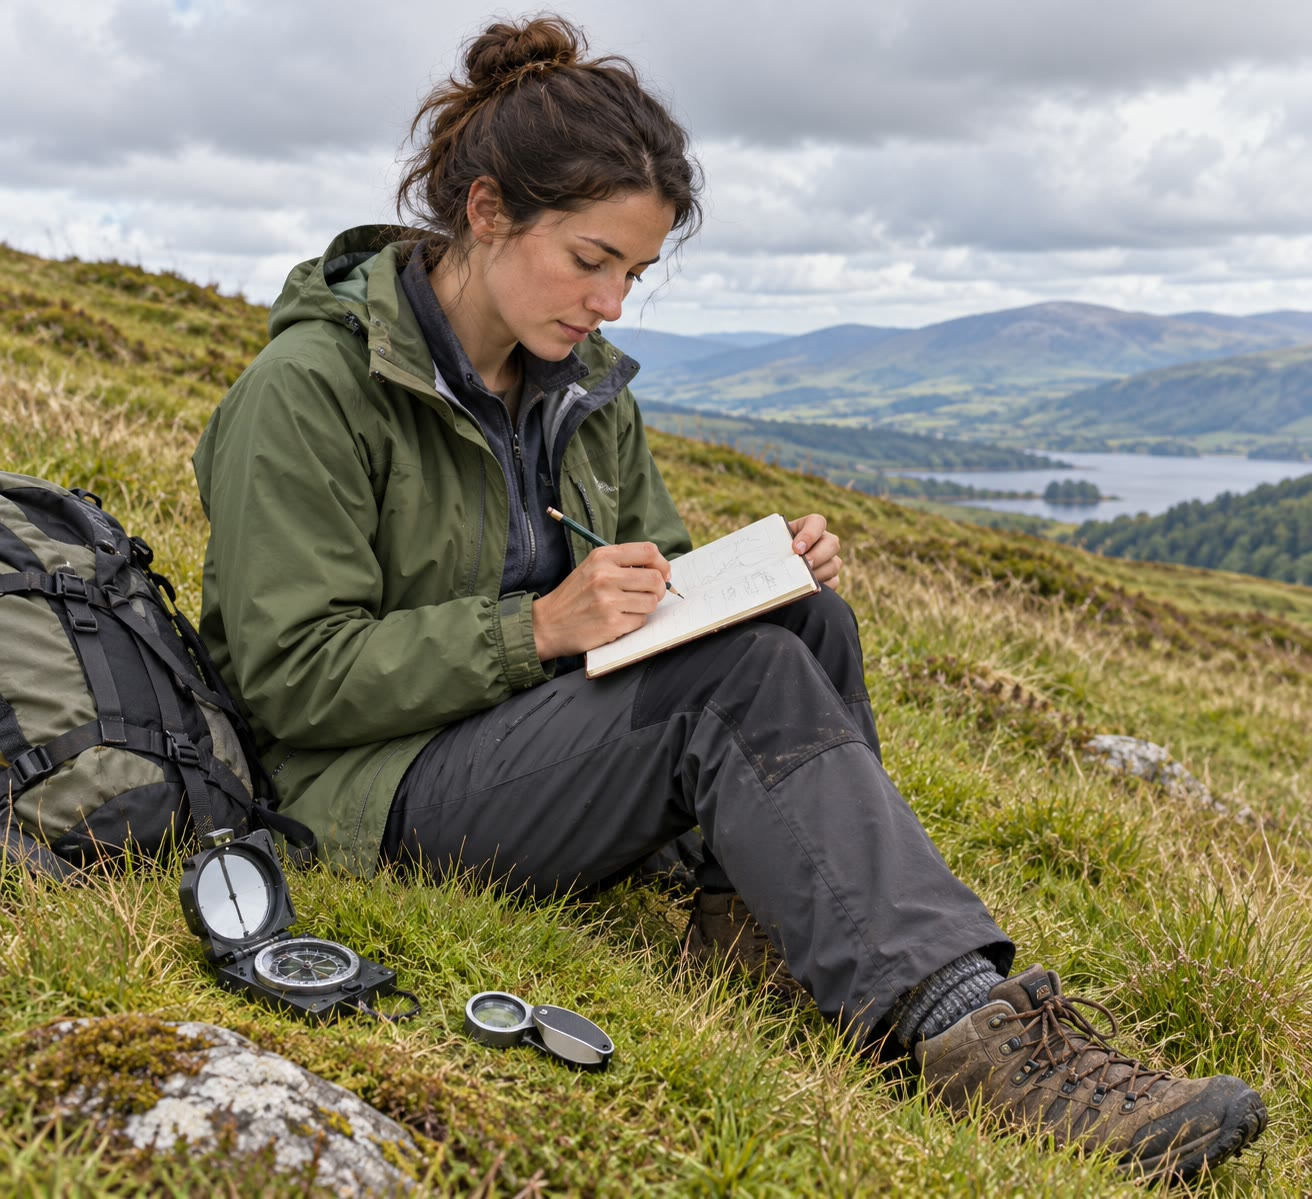
\includegraphics[width=\linewidth]{images/book3/ai/b1-field-notebook.jpg}
\end{minipage}
\end{inthefield}

\section{产状的测量}

平面的\omterm{def:b1:geological-maps:attitude}{产状}——岩层、断层或节理——用
罗盘测斜仪测量：磁罗盘用于读取\omterm{def:b1:spherical-astronomy:horizontal}{方位角}，摆或水准器用于读取
与水平面的夹角。将其边缘沿地面\omterm{def:b1:geological-maps:attitude}{走向}放置以读取\omterm{def:b1:geological-maps:attitude}{走向}，
或将仪器置于地面的最陡线上以读取\omterm{def:b1:geological-maps:attitude}{倾角}，
并由该线的\omterm{def:b1:spherical-astronomy:horizontal}{方位角}确定
\omterm{def:b1:geological-maps:attitude}{倾向}。

\begin{omfigure}
\begin{tikzpicture}[font=\scriptsize]
% (a) plan view
\begin{scope}
\fill[icsJurassic!25] (0,0) -- (3.6,0.5) -- (3.9,2.9) -- (0.3,2.4) -- cycle;
\draw (0,0) -- (3.6,0.5) -- (3.9,2.9) -- (0.3,2.4) -- cycle;
\draw[omDef, thick] (0.4,1.55) -- (3.5,1.98);
\node[omDef, above, rotate=8, fill=icsJurassic!25, inner sep=1pt] at (0.95,1.65) {走向线};
% compass box laid along the strike line
\begin{scope}[shift={(2.5,1.84)}, rotate=8]
\draw[fill=white] (-0.6,0) rectangle (0.6,0.32);
\draw (0,0.16) circle (0.12);
\end{scope}
\draw[omThm, thick, -{Stealth[length=2mm]}] (1.6,1.71) -- (1.75,0.62);
\node[omThm, right, fill=icsJurassic!25, inner sep=1pt] at (1.78,0.85) {倾向};
\node[below, align=center] at (1.95,-0.15) {(a) 平面图：罗盘边缘 \\ 沿走向放置};
\draw[->] (4.3,1.6) -- (4.3,2.4) node[above] {北};
\end{scope}
% (b) side view, vertical section along the dip direction
\begin{scope}[xshift=5.8cm]
\fill[icsJurassic!25] (0,1.6) -- (3.6,0.2) -- (3.6,-0.3) -- (0,-0.3) -- cycle;
\draw[thick] (0,1.6) -- (3.6,0.2);
% clinometer resting on the surface
\begin{scope}[shift={(2.5,0.6278)}, rotate=-21.25]
\draw[fill=white] (-0.75,0) rectangle (0.75,0.3);
\draw (0,0.15) circle (0.11);
\draw[black!70] (0,0.15) -- ++(-68.75:0.11);
\end{scope}
% dip angle at the lower end of the surface
\coordinate (P) at (0.7,1.3278);
\draw[black!60] (P) -- ++(1.6,0) node[right] {水平};
\draw[omThm] ($(P)+(1.1,0)$) arc[start angle=0, end angle=-21.25, radius=1.1];
\node[omThm] at ($(P)+(0.9,-0.15)$) {$\delta$};
\node[below, align=center] at (1.8,-0.35) {(b) 沿倾向的剖面：\\ 罗盘测斜仪置于最陡线上};
\end{scope}
\end{tikzpicture}

{\small 测量\omterm{def:b1:geological-maps:attitude}{产状}（示意图）。(a) 罗盘边缘水平放在岩层上，
所得读数即为\omterm{def:b1:geological-maps:attitude}{走向}；\omterm{def:b1:geological-maps:attitude}{倾向}与之垂直，沿岩层向下。
(b) 将测斜仪竖立于其边缘，沿最陡线放置，
测得\omterm{def:b1:geological-maps:attitude}{倾角} $\delta$。}
\end{omfigure}

一条直线——例如\omterm{def:b1:geological-maps:fold}{褶皱轴}、断层面上的擦痕、卵石的
长轴——都有其自身的方位。

\begin{definition}[倾伏向与倾伏角]\label{def:b1:field-lab-methods-1:trend-plunge}
直线的\emph{倾伏向}\index{倾伏向}是其水平投影的\omterm{def:b1:spherical-astronomy:horizontal}{方位角}，
沿直线指向下方的那一端量取。
其\emph{倾伏角}\index{倾伏角}是直线与水平面之间的夹角，
在包含该直线的竖直面内量取。
朝 \ang{015} 方向倾伏 \ang{20} 的直线记作 $20\to015$。
\end{definition}

\omterm{def:b1:field-lab-methods-1:trend-plunge}{倾伏向}为 $t$、\omterm{def:b1:field-lab-methods-1:trend-plunge}{倾伏角}为 $p$ 的直线，其朝下的单位矢量
$(\cos p\sin t, \cos p\cos t, -\sin p)$，以东、北、上分量表示；
位于\omterm{def:b1:geological-maps:attitude}{倾向}为 $\alpha$、\omterm{def:b1:geological-maps:attitude}{倾角}为 $\delta$ 的平面内的直线，其\omterm{def:b1:field-lab-methods-1:trend-plunge}{倾伏角}
等于该平面在\omterm{def:b1:spherical-astronomy:horizontal}{方位角}为 $t$ 的竖直面内的\omterm{def:b1:cross-sections:apparent-dip}{视倾角}，因此
$\tan p = \tan\delta\cos(\alpha - t)$（见\cref{thm:b1:cross-sections:apparent-dip}）。

\subsection{磁偏角}

指南针的磁针指向磁北，而非地理北；两者之间的夹角
即磁偏角，磁北位于地理北以东时取正值。
本书的地图与\omterm{def:b1:geological-maps:attitude}{产状}
均采用地理\omterm{def:b1:spherical-astronomy:horizontal}{方位角}。

\begin{method}[校正指南针方位角]\label{met:b1:field-lab-methods-1:declination}
\begin{enumerate}
  \item 依据地球磁场模型，查得该地点、该日期的磁偏角 $D$
        （东偏为正，西偏为负）。
  \item 将其加到罗盘读得的每个\omterm{def:b1:spherical-astronomy:horizontal}{方位角}上：地理\omterm{def:b1:spherical-astronomy:horizontal}{方位角} $=$
        磁\omterm{def:b1:spherical-astronomy:horizontal}{方位角} $+ D$，并对 \ang{360} 取模。
  \item \omterm{def:b1:geological-maps:attitude}{倾角}与\omterm{def:b1:field-lab-methods-1:trend-plunge}{倾伏角}不作修改：它们是从水平面量取的，
        依据的是重力，而非磁针。
\end{enumerate}
多数野外罗盘可以机械地设定为加上 $D$；该设定值及其
所对应的年份，均记录在\omterm{def:b1:field-lab-methods-1:station}{野外记录簿}中。
\end{method}

\begin{dated}{2026}
% ledger: noaa:wmm-edinburgh, noaa:wmm-reykjavik, noaa:wmm-anchorage, noaa:wmm-wellington
2026 年 1 月 1 日，World Magnetic Model（2025 版）给出的
爱丁堡的磁偏角为 \ang{-0.47}（西偏），年变化量为
\ang{+0.20}；雷克雅未克为 \ang{-11.28}，年变化量为 \ang{+0.30}；
安克雷奇为 \ang{+14.20}（东偏），年变化量为 \ang{-0.28}；以及
惠灵顿为 \ang{+23.23}。一位忘记在惠灵顿做修正的地质学家，
会使每个\omterm{def:b1:spherical-astronomy:horizontal}{方位角}的误差超过 \ang{23}；一位沿用十年前爱丁堡设定值的
地质学家，则会带来约
\ang{2} 的误差。
\end{dated}

\subsection{重复测量}

单次测量层面的\omterm{def:b1:geological-maps:attitude}{产状}带有误差：层面从来不是
理想的平面，仪器也不可能完全校准，读数还要
按度取整。因此，地质学家会对同一层面多次测量，
或对同一翼上的若干层面测量，再取平均。对\omterm{def:b1:spherical-astronomy:horizontal}{方位角}取平均时需要
格外小心：读数 \ang{355} 与 \ang{005} 所描述的两个方向相隔 \ang{10}，
但它们的算术平均 \ang{180} 却指向相反方向。正确的平均
方法应借助矢量进行。

\begin{definition}[平均方位（矢量平均）]\label{def:b1:field-lab-methods-1:mean-orientation}
对\omterm{def:b1:geological-maps:attitude}{倾向}为 $\alpha$、\omterm{def:b1:geological-maps:attitude}{倾角}为 $\delta$ 的平面，令
\[
  \vec n = (\sin\delta\sin\alpha,\ \sin\delta\cos\alpha,\ \cos\delta)
\]
为其朝上的单位法向量（东、北、上分量）。
\emph{平均方位}\index{平均方位}（或\emph{矢量平均}）是 $N$ 个读数的
法向量 $\vec n_1, \dots, \vec n_N$ 所对应的平面，即法向量为
$\vec m = \vec S/\|\vec S\|$ 的平面，$\vec S = \sum_i \vec n_i$ 为它们的
合向量；$\bar R = \|\vec S\|/N$ 即\emph{平均合向量长度}。
平均\omterm{def:b1:geological-maps:attitude}{倾向}与平均\omterm{def:b1:geological-maps:attitude}{倾角}分别为 $\bar\alpha = \operatorname{atan2}(S_E, S_N)$
与 $\bar\delta = \arccos(S_U/\|\vec S\|)$。
\end{definition}

由\cref{ch:b1:geological-maps}可知，$\vec n$ 即为法向量：
平面 $z = -\tan\delta\,(x\sin\alpha + y\cos\alpha)$ 的向上法向量为
$(\tan\delta\sin\alpha, \tan\delta\cos\alpha, 1)$，其长度为
$1/\cos\delta$。

\begin{proposition}[矢量平均即最接近的方向]\label{prop:b1:field-lab-methods-1:vector-mean}
在所有单位矢量 $\vec u$ 中，平均法向量 $\vec m$ 使
$\sum_i \vec n_i\cdot\vec u = \sum_i \cos\theta_i(\vec u)$ 达到最大，其中
$\theta_i(\vec u)$ 为 $\vec n_i$ 与 $\vec u$ 的夹角；等价地，
它使 $\sum_i \|\vec n_i - \vec u\|^2$ 达到最小。此外
\[
  \bar R = \frac1N\sum_i \cos\theta_i, \qquad \theta_i = \theta_i(\vec m),
\]
因此 $0 < \bar R \le 1$，且仅当所有读数一致时 $\bar R = 1$，并且
当散布较小时，读数与其平均之间的方均根夹角
为
\[
  \theta_{\text{rms}} \approx \sqrt{2(1 - \bar R)} \quad\text{（弧度）}.
\]
\end{proposition}

\begin{proof}
$\sum_i \vec n_i\cdot\vec u = \vec S\cdot\vec u \le \|\vec S\|$ 由
柯西–施瓦茨不等式，当且仅当 $\vec u = \vec m$ 时取等号。
由于 $\|\vec n_i - \vec u\|^2 = 2 - 2\,\vec n_i\cdot\vec u$，两个问题
实质相同。取 $\vec u = \vec m$ 时上界可以取到：
$\|\vec S\| = \sum_i\cos\theta_i$，即 $\bar R$ 的表达式。最后
$\cos\theta \approx 1 - \theta^2/2$ 在 $\theta$ 很小时成立，因此 $1 - \bar R \approx
\frac1N\sum_i\theta_i^2/2 = \theta_{\text{rms}}^2/2$。
\end{proof}

两个角度上的误差如何使法线移动？对 $\vec n$ 求导，
\[
  \frac{\partial\vec n}{\partial\delta} = (\cos\delta\sin\alpha,\ \cos\delta\cos\alpha,\ -\sin\delta),
  \qquad
  \frac{\partial\vec n}{\partial\alpha} = (\sin\delta\cos\alpha,\ -\sin\delta\sin\alpha,\ 0):
\]
第一个偏导向量长度为 1，第二个长度为 $\sin\delta$，二者
互相垂直。因此微小误差 $\Delta\delta$ 与 $\Delta\alpha$ 使
法线转过的角度为
\[
  \Delta\theta \approx \sqrt{\Delta\delta^2 + \sin^2\delta\,\Delta\alpha^2}.
\]
在\omterm{def:b1:geological-maps:attitude}{倾角}平缓的岩层上，\omterm{def:b1:geological-maps:attitude}{倾向}误差几乎不改变
平面：对\omterm{def:b1:geological-maps:attitude}{倾角}为 \ang{12} 的岩层，\ang{3} 的\omterm{def:b1:geological-maps:attitude}{倾向}误差使
平面仅转过 $3\sin\ang{12} = \ang{0.6}$。反过来，这正是野外
地质学家的难题：平缓岩层的\omterm{def:b1:geological-maps:attitude}{倾向}很难由其
平面确定，地表的细微起伏会使其大幅散布。
对 $N$ 个独立读数取平均，每个读数的标准差为
$s$，则平均值的标准误差为 $s/\sqrt N$（数学）：要使其减半，所需读数数量须增至
原来的四倍。

\begin{omfigure}
\begin{tikzpicture}
\begin{axis}[name=dd, width=0.47\linewidth, height=4.6cm, ybar, bar width=0.8,
  xmin=72.5, xmax=88.5, ymin=0, ymax=8.5, ytick={0,2,4,6,8},
  tick label style={font=\scriptsize}, label style={font=\small},
  xlabel={倾向 (\si{\degree})}, ylabel={读数}]
\addplot[fill=icsJurassic!40, draw=black] table[x=value, y=count] {figdata/out/bachelor-1-attitude_stats-hist-dd.dat};
\draw[omThm, thick] (axis cs:80.84,0) -- (axis cs:80.84,8.5);
\draw[omThm, densely dashed] (axis cs:77.91,0) -- (axis cs:77.91,8.5);
\draw[omThm, densely dashed] (axis cs:83.77,0) -- (axis cs:83.77,8.5);
\end{axis}
\begin{axis}[at={(dd.east)}, anchor=west, xshift=1.1cm, width=0.47\linewidth, height=4.6cm,
  ybar, bar width=0.8, xmin=5.5, xmax=18.5, ymin=0, ymax=8.5, ytick={0,2,4,6,8},
  tick label style={font=\scriptsize}, label style={font=\small},
  xlabel={倾角 (\si{\degree})}]
\addplot[fill=icsJurassic!40, draw=black] table[x=value, y=count] {figdata/out/bachelor-1-attitude_stats-hist-dip.dat};
\draw[omThm, thick] (axis cs:12.36,0) -- (axis cs:12.36,8.5);
\draw[omThm, densely dashed] (axis cs:10.24,0) -- (axis cs:10.24,8.5);
\draw[omThm, densely dashed] (axis cs:14.48,0) -- (axis cs:14.48,8.5);
\end{axis}
\end{tikzpicture}

{\small 瓦尔登东翼岩层层面的二十五次模拟读数，
其模型\omterm{def:b1:geological-maps:attitude}{产状}为 $080.7/12.2$，两个角度上各附有标准差为 \ang{3} 的误差，
取整到度。实线：平均值；虚线：
两侧各一个标准差（$080.8 \pm 2.9$ 与 $12.4 \pm 2.1$）。
这 25 个读数的矢量平均为 $080.9/12.3$。}
\end{omfigure}

\section{手持放大镜与野外鉴定}

多数岩石在野外即可命名，无需等待实验室工作，依据
手持放大镜所见的矿物以及岩石的断裂方式。地质学家
观察新鲜的表面，因为风化会使岩石覆上一层并变色，并
记录颗粒的大小（肉眼可见、需借助放大镜，
或根本看不见）、颗粒的形状、颗粒是否像镶嵌那样相互咬合，
或像沙一样被胶结，以及有无任何定向排列。矿物
依据本章开头回顾的性质加以识别：石英的玻璃
光泽与无解理，长石的两组解理与暗
白色，云母呈片状，方解石具有菱面体解理。
硬度用钢针来检验：石英比钢硬，
而方解石则软得多。

专业人员随身携带一小瓶稀盐酸滴瓶：
碳酸盐岩在滴落处会释放出二氧化碳气泡，
（化学）。方解石反应剧烈；白云石除非研磨成粉，否则反应微弱。
使用酸时须佩戴手套与护目镜，且绝不可由本书读者
操作，此处所述仅为专业操作。

\section{样品}

\begin{definition}[定向样品]\label{def:b1:field-lab-methods-1:sample}
\emph{定向样品}\index{定向样品}是一种岩石样品，地质学家在将其采下前，
已在其一个表面上标出了\omterm{def:b1:geological-maps:attitude}{产状}，
即一条\omterm{def:b1:geological-maps:attitude}{走向}线与一个\omterm{def:b1:geological-maps:attitude}{倾向}箭头，或某条线的\omterm{def:b1:field-lab-methods-1:trend-plunge}{倾伏向}，
以便在实验室中将样品放回其野外原来的位置。
\end{definition}

样品只有在能代表其所对应的岩层单元时才有用——
新鲜、未风化、非取自岩脉或坠落岩块——且其
来源确定。每件样品都标注观测点编号和样品编号，
同时写在岩石和样品袋上，并在记录簿中登记
其位置、所属岩层单元以及采集原因。用于化学或
同位素分析的样品，其结果或许数十年后才会公布，
需以书面记录追踪样品自野外至实验室所经过的每一双手，
即一条保管链——以确保不致对哪块岩石
对应哪个编号存疑。凡岩石内部某种事物的方向很重要时，
均需\omterm{def:b1:field-lab-methods-1:sample}{定向样品}，例如矿物的定向排列，
显微镜下所见的组构，或
岩石形成时所获得的磁化方向。

\section{薄片与偏光显微镜}

\begin{definition}[薄片]\label{def:b1:field-lab-methods-1:thin-section}
\emph{薄片}\index{薄片}是一片岩石切片，粘贴在
载玻片上，并磨至标准厚度 \qty{30}{\micro\metre}，
足以使大多数矿物透光。
\end{definition}

\begin{inthelab}[制作薄片]
% ledger: jaic:thin-section, jaic:epoxy-ri
\begin{minipage}[t]{0.58\linewidth}\vspace{0pt}
在制样实验室中，技术员用金刚石锯从
样品上切下一小块，将其一面磨得十分平整，并用
环氧树脂将其粘在载玻片上，该树脂的折射率为 1.54 至 1.55，
与石英的折射率几乎相同。随后锯去大部分岩块，并将\omterm{def:b1:field-lab-methods-1:thin-section}{薄片}
在旋转研磨盘上用越来越细的磨料继续磨削，直至
厚度为 \qty{30}{\micro\metre}。技术员在
显微镜下依据石英颗粒所呈现的干涉色（\cref{ch:b1:optical-mineralogy}）检查厚度，
并以薄盖玻片或抛光面收尾。多孔或易碎的
岩石先要用树脂浸渍，使其保持完整。
\end{minipage}\hfill
\begin{minipage}[t]{0.39\linewidth}\vspace{0pt}
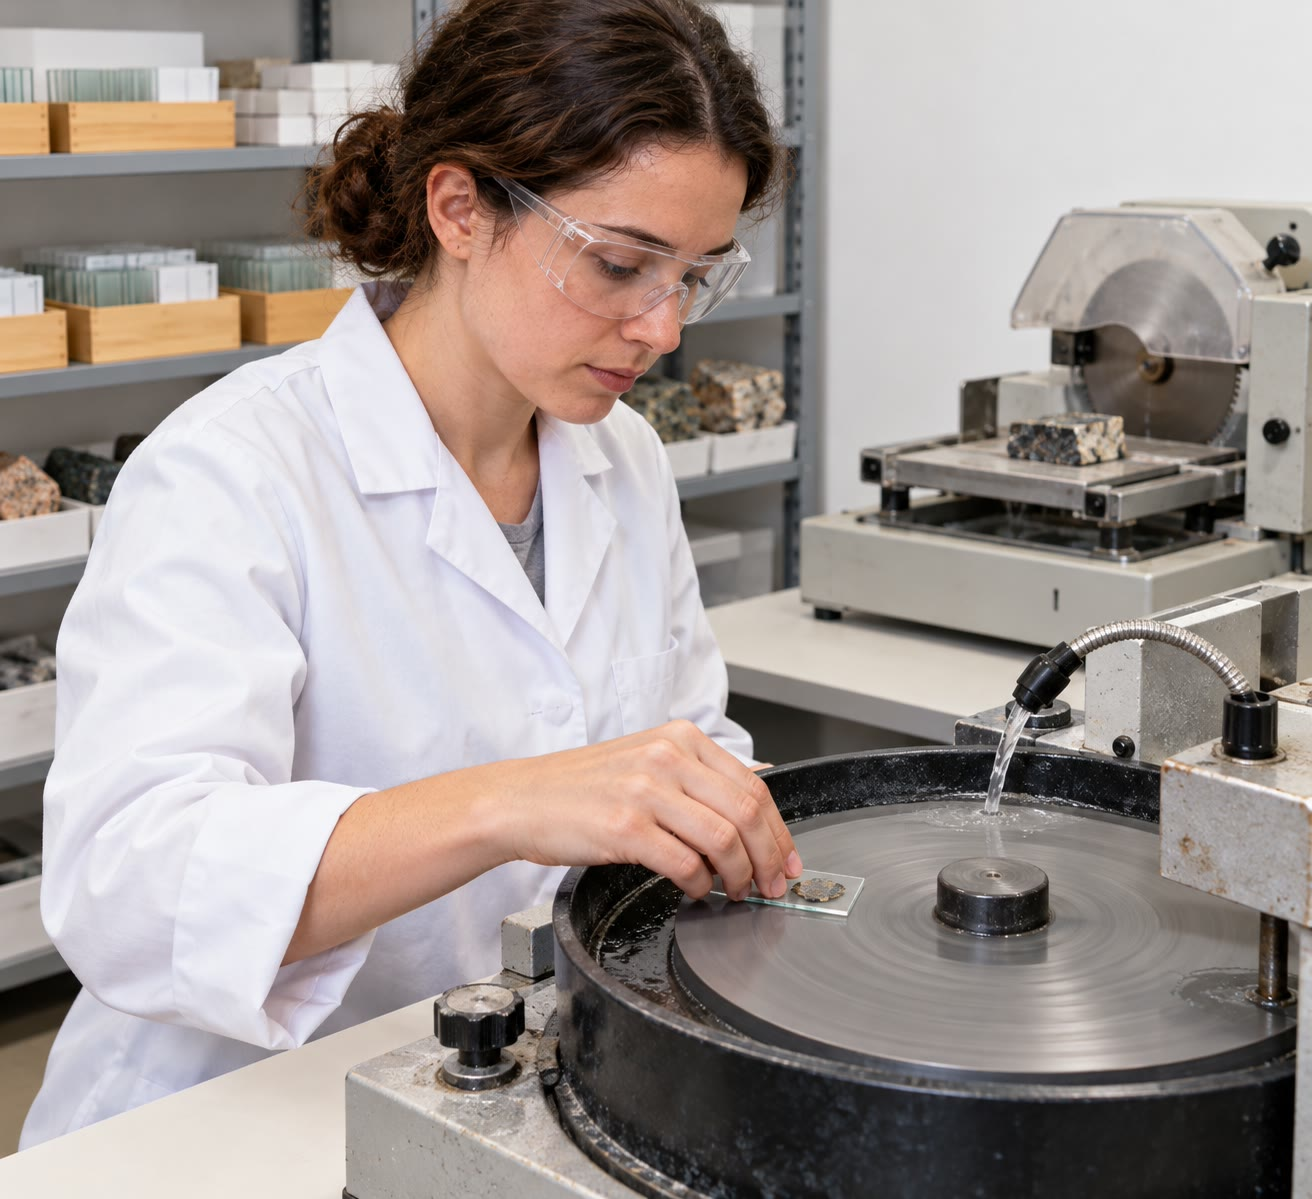
\includegraphics[width=\linewidth]{images/book3/ai/b1-thin-section-lab.jpg}
\end{minipage}
\end{inthelab}

\omterm{def:b1:field-lab-methods-1:thin-section}{薄片}在装有两块偏振
滤光片的显微镜下研究。线偏振是物理学的内容：这里只需
知道偏振滤光片只透过沿一个方向振动的光，
而两块互相垂直放置的滤光片什么光也透不过。

\begin{definition}[偏光显微镜、单偏光、正交偏光]\label{def:b1:field-lab-methods-1:microscope}
称\emph{偏光显微镜}\index{偏光显微镜}为一种透射光显微镜，
其载物台下方装有偏振滤光片（起偏器），载物台
可在刻度尺上转动 \ang{360}；物镜与目镜之间装有第二块偏振滤光片（检偏器），
可移入或移出光路，
其振动方向与起偏器的振动方向互相垂直。
检偏器移出时，样品在
\emph{单偏光}\index{单偏光}下观察；检偏器移入时，
样品在\emph{正交偏光}\index{正交偏光}之间观察。
\end{definition}

\begin{omfigure}
\begin{tikzpicture}[font=\scriptsize, x=1cm, y=0.62cm]
\def\comp#1#2#3{\draw[fill=#3] (-1.1,#1-0.18) rectangle (1.1,#1+0.18); \node[right] at (1.3,#1) {#2};}
\draw[omThm!60, line width=3pt, -{Stealth[length=3mm]}] (0,0.3) -- (0,10.6);
\draw[fill=yellow!40] (0,0) circle (0.3); \node[right] at (1.3,0) {光源};
\comp{1.3}{起偏器：只透过一个振动方向的光}{omDef!25}
\draw[omDef, thick, <->] (-0.5,1.3) -- (0.5,1.3);
\draw[fill=white] (-1.0,2.3) .. controls (0,2.75) .. (1.0,2.3) .. controls (0,1.85) .. (-1.0,2.3);
\node[right] at (1.3,2.3) {聚光器};
\draw[fill=black!70] (-1.6,3.4) rectangle (1.6,3.55);
\draw[fill=icsJurassic!40] (-0.5,3.55) rectangle (0.5,3.65);
\node[right] at (1.7,3.48) {带刻度的旋转载物台与薄片};
\draw[fill=white] (-0.45,4.5) rectangle (0.45,5.4); \node[right] at (1.3,4.95) {物镜};
\comp{6.2}{附件插槽}{black!10}
\comp{7.2}{检偏器：移入（正交偏光）或移出（单偏光）}{omDef!25}
\draw[omDef, thick, <->] (0,6.85) -- (0,7.55);
\comp{8.2}{贝特兰透镜（可选）}{black!5}
\draw[fill=white] (-0.35,9.1) rectangle (0.35,10.0); \node[right] at (1.3,9.55) {带十字丝的目镜};
\end{tikzpicture}

{\small \omterm{def:b1:field-lab-methods-1:microscope}{偏光显微镜}的光路（示意图，自下而上）。
起偏器与检偏器的振动方向互相垂直（双箭头）；
两者之间无物体时，\omterm{def:b1:field-lab-methods-1:microscope}{正交偏光}下视场呈黑色。}
\end{omfigure}

\omterm{def:b1:field-lab-methods-1:microscope}{正交偏光}之间，载玻片的玻璃、环氧树脂及任何均质
矿物（即光学性质在各方向都相同的矿物，例如
立方晶体）在载物台任意旋转时都保持黑色。大多数矿物
并非均质：它们会改变穿过的光的偏振状态，
并呈现随载物台转动而变化的干涉色，
载物台转动一周时干涉色消光四次。它们为何如此，以及颜色与角度如何
用于鉴定矿物，在\cref{ch:b1:optical-mineralogy}中讨论。
\omterm{def:b1:field-lab-methods-1:thin-section}{薄片}中的矿物通常在约
$16\times$ 至 $400\times$ 的放大倍率下观察。
% ledger: jaic:magnification

\begin{omfigure}
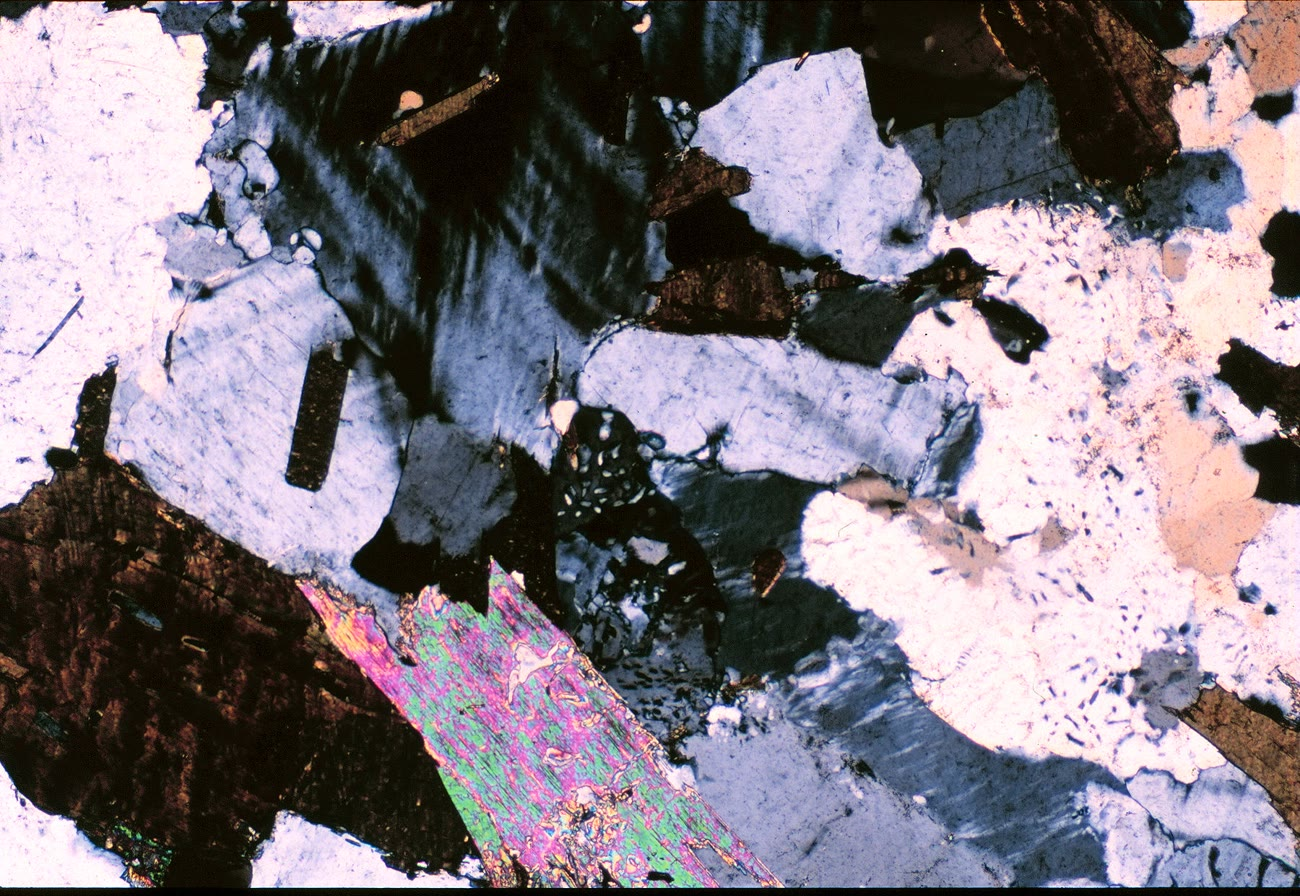
\includegraphics[width=0.55\linewidth]{images/book3/b1-granite-thin-section-xpl.jpg}
% ledger: commons:granite-xpl

{\small \omterm{def:b1:field-lab-methods-1:microscope}{正交偏光}下的花岗岩\omterm{def:b1:field-lab-methods-1:thin-section}{薄片}。黑云母呈棕色，
白云母呈亮粉色与绿色干涉色，斜长石因双晶而呈条纹，
石英呈白色至灰色。照片：Darla
Sondrol, CC0（维基共享资源）。}
\end{omfigure}

\begin{safety}
野外与实验室工作的安全，靠的是专业规范，而非运气。
在野外，地质学家应结伴工作，或留下书面的路线计划
及预计返回时间；随身携带天气预报、地图和急救用品，远离
悬崖及采石场崖面的坡脚与边缘，并在任何岩石可能坠落或
碎裂之处，戴安全帽并佩戴护目装备；在活动场地作业，
须遵守操作人员的规定。实验室中，切割锯与研磨盘
均加防护罩并通水以抑制粉尘，树脂与酸
在通风橱内操作，须戴手套和护目镜，每种化学品都备有安全技术说明书。
上述这些做法并非只为本书读者而设：本章
所描述的是专业实践。
\end{safety}

\section{练习}

\begin{exercise}[$\star$]\label{exo:b1:field-lab-methods-1:1}
卫星接收机给出的位置误差在约 \qty{4.9}{m} 以内。
求该误差在比例尺为 1:10\,000 的地图上相当于多大，在 1:25\,000 的地图上又为多大？
\end{exercise}

\begin{exercise}[$\star$]\label{exo:b1:field-lab-methods-1:2}
一台未设置磁偏角的指南针在某岩层上读得\omterm{def:b1:geological-maps:attitude}{倾向}
为 \ang{052}。若该读数于 2026 年 1 月 1 日在雷克雅未克测得，求其地理\omterm{def:b1:geological-maps:attitude}{倾向}；
若同日改在惠灵顿测得，结果又如何（带日期的方框）。
\end{exercise}

\begin{exercise}[$\star$]\label{exo:b1:field-lab-methods-1:3}
某\omterm{def:b1:geological-maps:fold}{褶皱轴}以 \ang{20} 的\omterm{def:b1:field-lab-methods-1:trend-plunge}{倾伏角}朝 \ang{015} 方向倾伏，按正文的
方式写出其\omterm{def:b1:geological-maps:attitude}{产状}，并以东、北、上三个分量给出其向下的单位矢量。
\end{exercise}

\begin{exercise}[$\star$]\label{exo:b1:field-lab-methods-1:4}
某竖直节理三次读数得其法线的\omterm{def:b1:spherical-astronomy:horizontal}{方位角}分别为 \ang{350}、
\ang{358} 和 \ang{006}。求它们的算术平均值，然后求
这三个水平单位矢量之和的\omterm{def:b1:spherical-astronomy:horizontal}{方位角}。哪一种平均值是正确的？
\end{exercise}

\begin{exercise}[$\star\star$]\label{exo:b1:field-lab-methods-1:5}
某一岩层\omterm{def:b1:geological-maps:attitude}{倾角}的五次读数分别为 \ang{34}、\ang{37}、\ang{35}、
\ang{33} 和 \ang{36}。求其平均值、标准差以及
平均值的标准误。
\end{exercise}

\begin{exercise}[$\star\star$]\label{exo:b1:field-lab-methods-1:6}
一位地质学家在对称\omterm{def:b1:geological-maps:fold}{褶皱}的两翼各取一个读数并求平均：$090/30$
和 $270/30$。求矢量平均与 $\bar R$。问题出在哪里？
\end{exercise}

\begin{exercise}[$\star\star$]\label{exo:b1:field-lab-methods-1:7}
  擦痕位于\omterm{def:b1:geological-maps:attitude}{产状}为 $080/12$ 的层面上，其\omterm{def:b1:field-lab-methods-1:trend-plunge}{倾伏向}为
  \ang{120}。其\omterm{def:b1:field-lab-methods-1:trend-plunge}{倾伏角}为多少？若\omterm{def:b1:field-lab-methods-1:trend-plunge}{倾伏向}为 \ang{170}，\omterm{def:b1:field-lab-methods-1:trend-plunge}{倾伏角}又为多少？
\end{exercise}

\begin{exercise}[$\star\star$]\label{exo:b1:field-lab-methods-1:8}
爱丁堡的磁偏角在 2026 年 1 月 1 日为 \ang{-0.47}，并且
每年变化 \ang{+0.20}。假设变化保持稳定，磁偏角何时
为零？2030 年 1 月 1 日时它是多少？
\end{exercise}

\begin{exercise}[$\star\star$]\label{exo:b1:field-lab-methods-1:9}
同一层的三个读数分别为 $080/10$、$080/12$ 和 $080/14$。证明其
矢量平均为 $080/12$，计算 $\bar R$，以及
$\sqrt{2(1 - \bar R)}$ 为 $\theta_{\text{rms}}$ 的估计值，并与精确的
方均根角相比较。
\end{exercise}

\begin{exercise}[$\star\star\star$]\label{exo:b1:field-lab-methods-1:10}
一张\omterm{def:b1:field-lab-methods-1:thin-section}{薄片}切过半径为 $r$ 的球形颗粒，切面距其球心的距离为 $h$，
$h$ 在 0 与 $r$ 之间任意取值且等可能。证明切面中所见圆的
平均半径为 $\pi r/4$。直径为 \qty{0.50}{mm} 的石英颗粒在\omterm{def:b1:field-lab-methods-1:thin-section}{薄片}中
平均看起来有多大？
\end{exercise}

\begin{exercise}[$\star\star\star$]\label{exo:b1:field-lab-methods-1:11}
证明：若一组读数的每个\omterm{def:b1:geological-maps:attitude}{倾向}都增加同一角度 $D$，
则其矢量平均的\omterm{def:b1:geological-maps:attitude}{倾向}增加 $D$，而\omterm{def:b1:geological-maps:attitude}{倾角}不变。
这对磁偏角校正为何重要？
\end{exercise}

\begin{exercise}[$\star\star\star$]\label{exo:b1:field-lab-methods-1:12}
在\omterm{def:b1:geological-maps:attitude}{倾角}为 \ang{12} 的层面上，单个读数的法向量在两个相互垂直的
方向上的标准差均为 \ang{2}：沿最大倾斜线方向的离散改变\omterm{def:b1:geological-maps:attitude}{倾角}，
垂直于它的方向的离散改变\omterm{def:b1:geological-maps:attitude}{倾向}。要使平均\omterm{def:b1:geological-maps:attitude}{倾角}的标准误差为
\ang{0.5}，需要多少个读数？
要使平均\omterm{def:b1:geological-maps:attitude}{倾向}的标准误差为 \ang{1}，又需要多少个读数？
\end{exercise}

\section{问题：瓦尔登东翼的野外工作季}

\begin{problem}[{周末问题——对十二个罗盘读数求平均，测量其离散程度，
校正这些读数，并与钻孔资料进行比较}]
\label{pb:b1:field-lab-methods-1:1}
% readings: figdata/bachelor-1/attitude_stats.py (part normals); values: calc/ch06.py
一位地质学家在瓦尔登\omterm{def:b1:geological-maps:fold}{背斜}东翼
的十二个测站测量层理，罗盘已按磁偏角设置，读数精确到
度。表中给出每个读数（\omterm{def:b1:geological-maps:attitude}{倾向}/\omterm{def:b1:geological-maps:attitude}{倾角}）及其
向上单位法向量 $\vec n = (n_E, n_N, n_U)$ 的分量，精确到小数点后四位。
\begin{center}
\small
\begin{tabular}{rcccc@{\qquad}rcccc}
\hline
 & 读数 & $n_E$ & $n_N$ & $n_U$ & & 读数 & $n_E$ & $n_N$ & $n_U$ \\
\hline
1 & $076/11$ & 0.1851 & 0.0462 & 0.9816 & 7 & $083/11$ & 0.1894 & 0.0233 & 0.9816 \\
2 & $081/13$ & 0.2222 & 0.0352 & 0.9744 & 8 & $083/12$ & 0.2064 & 0.0253 & 0.9781 \\
3 & $078/16$ & 0.2696 & 0.0573 & 0.9613 & 9 & $085/12$ & 0.2071 & 0.0181 & 0.9781 \\
4 & $081/11$ & 0.1885 & 0.0298 & 0.9816 & 10 & $078/11$ & 0.1866 & 0.0397 & 0.9816 \\
5 & $076/10$ & 0.1685 & 0.0420 & 0.9848 & 11 & $081/13$ & & & \\
6 & $083/14$ & 0.2401 & 0.0295 & 0.9703 & 12 & $082/11$ & & & \\
\hline
\end{tabular}
\end{center}

\medskip
\noindent\textbf{第一部分——平均\omterm{def:b1:geological-maps:attitude}{产状}。}
\begin{enumerate}
  \item 分别计算十二个\omterm{def:b1:geological-maps:attitude}{倾向}的算术平均值，
        以及十二个\omterm{def:b1:geological-maps:attitude}{倾角}的算术平均值。
  \item 举出两个读数，使其\omterm{def:b1:geological-maps:attitude}{倾向}的算术平均值毫无意义，
        并说明为何在此处这样做是合理的。
  \item 证明 $\vec n = (\sin\delta\sin\alpha, \sin\delta\cos\alpha,
        \cos\delta)$ 是一个单位向量，且与平面
        $\alpha/\delta$ 的倾斜线与\omterm{def:b1:geological-maps:attitude}{走向}线均垂直。
  \item 补全读数 11 和 12 的表格。
  \item 计算十二个法向量的合矢量 $\vec S$。
  \item 计算 $\|\vec S\|$ 及平均合向量长度 $\bar R$。
  \item 由此推出矢量平均：其\omterm{def:b1:geological-maps:attitude}{倾向}与\omterm{def:b1:geological-maps:attitude}{倾角}。
\end{enumerate}

\medskip
\noindent\textbf{第二部分——离散程度。}
\begin{enumerate}[resume]
  \item 计算\omterm{def:b1:geological-maps:attitude}{倾向}和\omterm{def:b1:geological-maps:attitude}{倾角}的
        样本标准差。
  \item 利用\cref{prop:b1:field-lab-methods-1:vector-mean}，估计
        读数与其平均值之间的方均根角 $\theta_{\text{rms}}$，
        以度为单位。
  \item 由第 8 题中两个标准差及本章的误差公式预测 $\theta_{\text{rms}}$，
        并进行比较。
  \item 两个标准差中哪一个对
        $\theta_{\text{rms}}$ 的贡献最大？为什么？
  \item 计算平均\omterm{def:b1:geological-maps:attitude}{倾角}与平均\omterm{def:b1:geological-maps:attitude}{倾向}的
        标准误差。
  \item \omterm{def:b1:geological-maps:attitude}{倾向}的离散程度 \ang{2.9} 是否说明测量粗心？
        请给出解释。
\end{enumerate}

\medskip
\noindent\textbf{第三部分——磁偏角。}
\begin{enumerate}[resume]
  \item 另一位地质学家忘记设置磁偏角，她的十二个读数
        在磁\omterm{def:b1:spherical-astronomy:horizontal}{方位角}下的矢量平均为 $083.1/12.1$。假设当年瓦尔登丘陵的
        磁偏角为西偏 \ang{2.5}。
        求她的平均值在地理\omterm{def:b1:spherical-astronomy:horizontal}{方位角}下的数值。
  \item 为什么她的平均\omterm{def:b1:geological-maps:attitude}{倾角}无需校正即是正确的？
  \item 她能否在求平均前逐个校正读数，而非
        校正平均值？这是否改变结果（见\cref{exo:b1:field-lab-methods-1:11}）？
  \item 十年后，一名学生沿用她的磁偏角设置，而此时磁偏角
        每年已变化 \ang{0.2}。误差有多大，
        与第 12 题的标准误差相比如何？
  \item 按右手定则给出第一位地质学家
        平均\omterm{def:b1:geological-maps:attitude}{产状}的\omterm{def:b1:geological-maps:attitude}{走向}。
\end{enumerate}

\medskip
\noindent\textbf{第四部分——罗盘与钻孔。}
\begin{enumerate}[resume]
  \item 在\cref{ch:b1:geological-maps}中，由三个钻孔求得石灰岩底面的
        \omterm{def:b1:geological-maps:attitude}{产状}为 $080.6/12.2$。将其与第 7 题的矢量平均
        按\omterm{def:b1:geological-maps:attitude}{倾向}与\omterm{def:b1:geological-maps:attitude}{倾角}逐项比较。
  \item 计算两个法向量之间的夹角。
  \item 平均方向的标准误差约为
        $\theta_{\text{rms}}/\sqrt N$，
        第 20 题中的差值是否显著？
  \item 需要多少个读数，才能使该标准误差减半？
  \item 请列举两种无论增加多少读数都无法减小的误差。
  \item 由十二个读数求东翼的平均\omterm{def:b1:geological-maps:attitude}{产状}，
        以\omterm{def:b1:geological-maps:attitude}{倾向}/\omterm{def:b1:geological-maps:attitude}{倾角}的形式给出，精确到度。
\end{enumerate}
\end{problem}
